\documentclass[
%% TIKZ_CLASSOPTION %%
tikz
]{standalone}
\usepackage{amsmath}
\usetikzlibrary{matrix}
%% EXTRA_TIKZ_PREAMBLE_CODE %%
\begin{document}
%% TIKZ_CODE %%
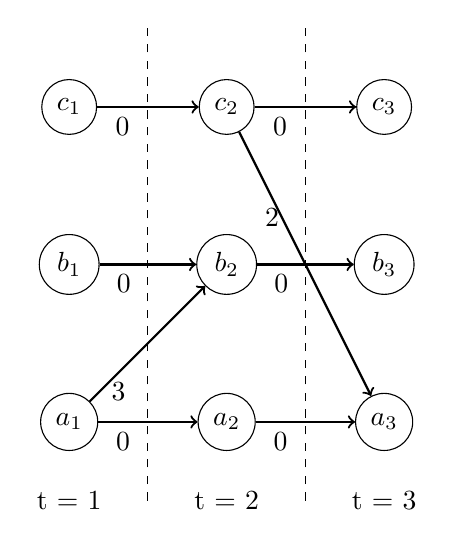
\begin{tikzpicture}

\tikzset{vertex/.style = {shape=circle,draw,minimum size=1.5em}}
\tikzset{edge/.style = {->,> = latex}}

\node[vertex] (a1) at (0,-1) {$a_{1}$};
\node[vertex] (b1) at (0,1) {$b_{1}$};
\node[vertex] (c1) at (0,3) {$c_{1}$};

\draw[dashed] (1,-2)--(1,4);

\node[vertex] (a2) at (2,-1) {$a_{2}$};
\node[vertex] (b2) at (2, 1) {$b_{2}$};
\node[vertex] (c2) at (2, 3) {$c_{2}$};

\draw[dashed] (3,-2)--(3,4);

\node[vertex] (a3) at (4,-1) {$a_{3}$};
\node[vertex] (b3) at (4,1) {$b_{3}$};
\node[vertex] (c3) at (4,3) {$c_{3}$};

\draw[->, thick] (a1) -> node[near start, below] {0} (a2);
\draw[->, thick] (a2) -> node[near start, below] {0} (a3);
\draw[->, thick] (b1) -> node[near start, below] {0} (b2);
\draw[->, thick] (b2) -> node[near start, below] {0} (b3);
\draw[->, thick] (c1) -> node[near start, below] {0} (c2);
\draw[->, thick] (c2) -> node[near start, below] {0} (c3);
\draw[->, thick] (a1) -> node[near start, below] {3} (b2);
\draw[->, thick] (c2) -> node[near start, below] {2} (a3);

\node at (0,-2) {t = 1};
\node at (2,-2) {t = 2};
\node at (4,-2) {t = 3};

\end{tikzpicture}
\end{document}
